Et verktøy for å visualisere hvordan gruppens medlemmer står i forhold til hverandre kalles samarbeidsindikatorer. 
Verktøyet er utarbeidet av Are Holden i samarbeid med EiT-staben. 
Dette var et tilbud alle gruppene i landsbyen fikk og testen ble gjennomført av fasilitatorene. 
Undersøkelsen ble gjennomført ved at vi svarte på en rekke spørsmål anonymt, disse svarene ble så grunnlaget for en graf som illustrerer hvordan gruppen ligger an.
Denne grafen belyser områder som gruppen har små, middels eller store utfordringer på. 
For å oppdage eventuell fremgang ble denne testen gjort to ganger iløpet av EiT-kurset. En gang helt i begynnelsen (2. landsbydag) og en gang mot slutten av prosjektet (10. landsbydag). 

\subsection{2. landsbydag}
På grunn av at den første testen ble tatt i en tidlig fase av gruppearbeidet, gir den et godt intrykk av gruppens initielle situasjon. 
På grafen er det to linjer, en heltrukken rød og en en striplet rød. 
Disse linjene markerer grensene på hvor ting blir regnet som store problemer og små problemer. 
\begin{figure}[H]
    \centering
    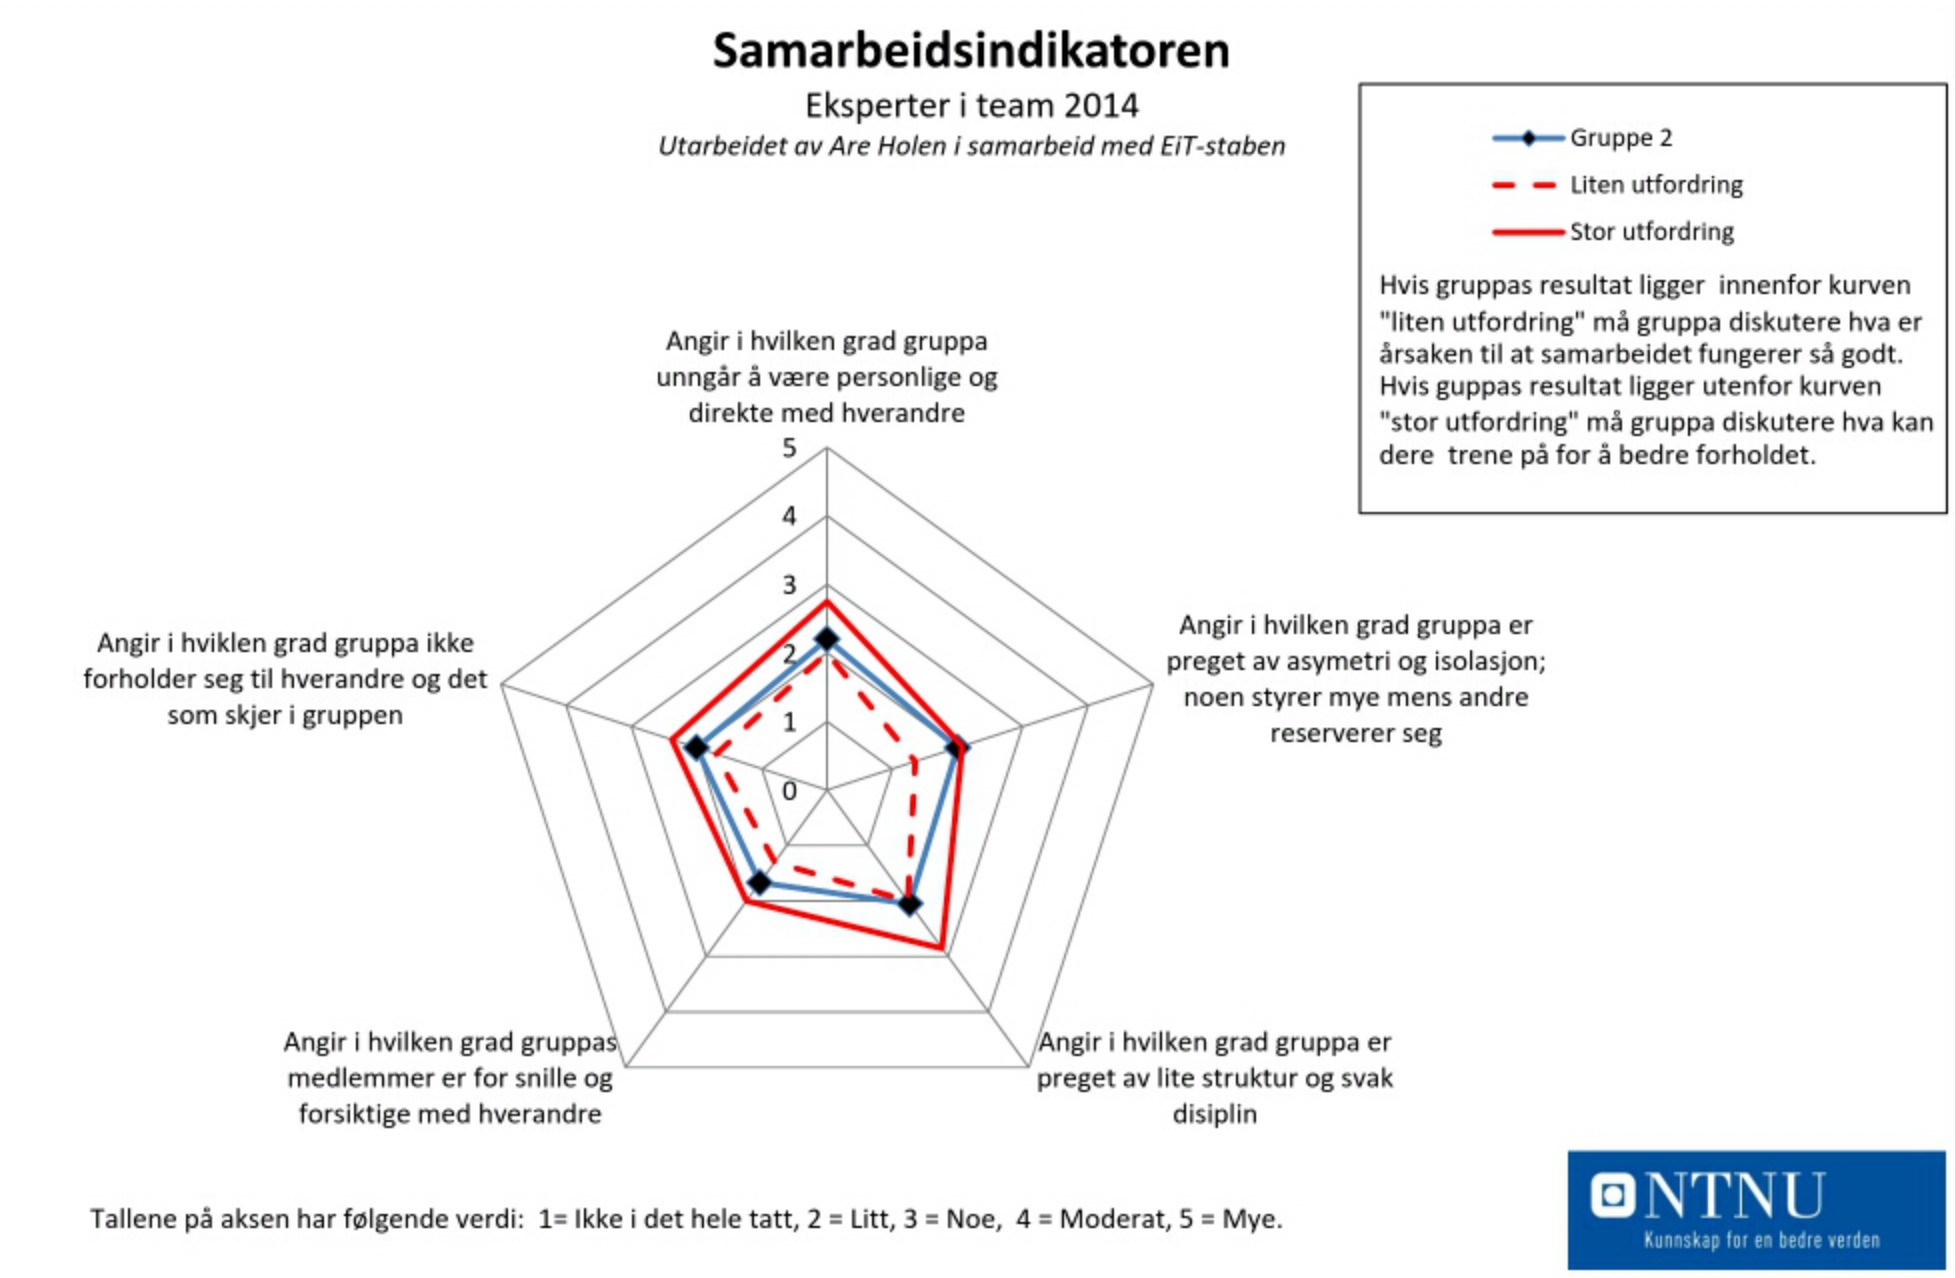
\includegraphics[width=0.7\textwidth]{images/samarbeidsindikator1.jpeg} 
    \caption{Samarbeidsindikatorer 2. landsbydag}
    \label{fig:sam1}
\end{figure}

\noindent \textbf{I hvilken grad gruppen unngår å være personlig:} 2.2.
\newline
\noindent Her hadde vi en moderat utfordring, noe som faller naturlig ettersom vi var en nydannet gruppe.
 At vi selv er bevisste på dette er et godt tegn, noe som gjenspeiler vårt fokus på dette området i videre prosessjobbing.
\vspace{\secspace}

\noindent \textbf{I hvilken grad gruppen er preget av asymetri og isolasjon:} 2.
\newline
\noindent Gruppen hadde de første dagene to medlemmer som var mest dominerende; Odd og Anders.
De tre resterende medlemmene hadde til da tatt en passiv posisjon og var ikke like aktive i felles aktiviterer. 
Under diskusjon av testens resultat, kom vi frem til at dette punktet er noe vi bør jobbe mye med. Vi definerte en aksjon, som var å rullere på å ha lederrollen i gruppa. 
Isolasjon er noe vi følte vi hadde lite av, så det passet dårlig at disse punktene var slått sammen. Vi har hele tiden lagt vekt på at alle i gruppen skal bli hørt, og tas seriøst. 

\vspace{\secspace}

\noindent \textbf{Hvilken grad gruppen er preget av lite struktur:} 1.
\newline
\noindent Som nevnt i punktet over tok noen tak og skapte rammer for arbeidet tidlig i prosessen. Dette gjorde at vi fra begynnelsen jobbet strukturert mot et felles mål. Vi var altså tidlig i prossessen preget av god struktur, og det viste seg i ettertid at grunnarbeidet gjort i den tidlige fasen la grunnlag for en god oppdeling av arbeidet. 
\vspace{\secspace}

\noindent \textbf{Hvilken grad gruppen er for snille med hverandre:} 1.8.
\newline
\noindent Vi kjente hverandre ikke så godt på dette tidspunktet, så dette kan virke naturlig. Vi satte likevel mål om å utvikle en trygghet og respekt for hverandre slik at det blir lettere å være ærlig og konstruktiv.
\vspace{\secspace}

\noindent \textbf{Hvilken grad gruppen ikke forholder seg til hverandre:} 1.
\newline
\noindent Vi hadde fra starten en god tone i gruppa, og ingen meldte seg ut eller ble fryst ut. Indikatoren viser her at dette ikke var et problem i noen særlig grad.

\subsection{10. landsbydag}
\begin{figure}[H]
    \centering
    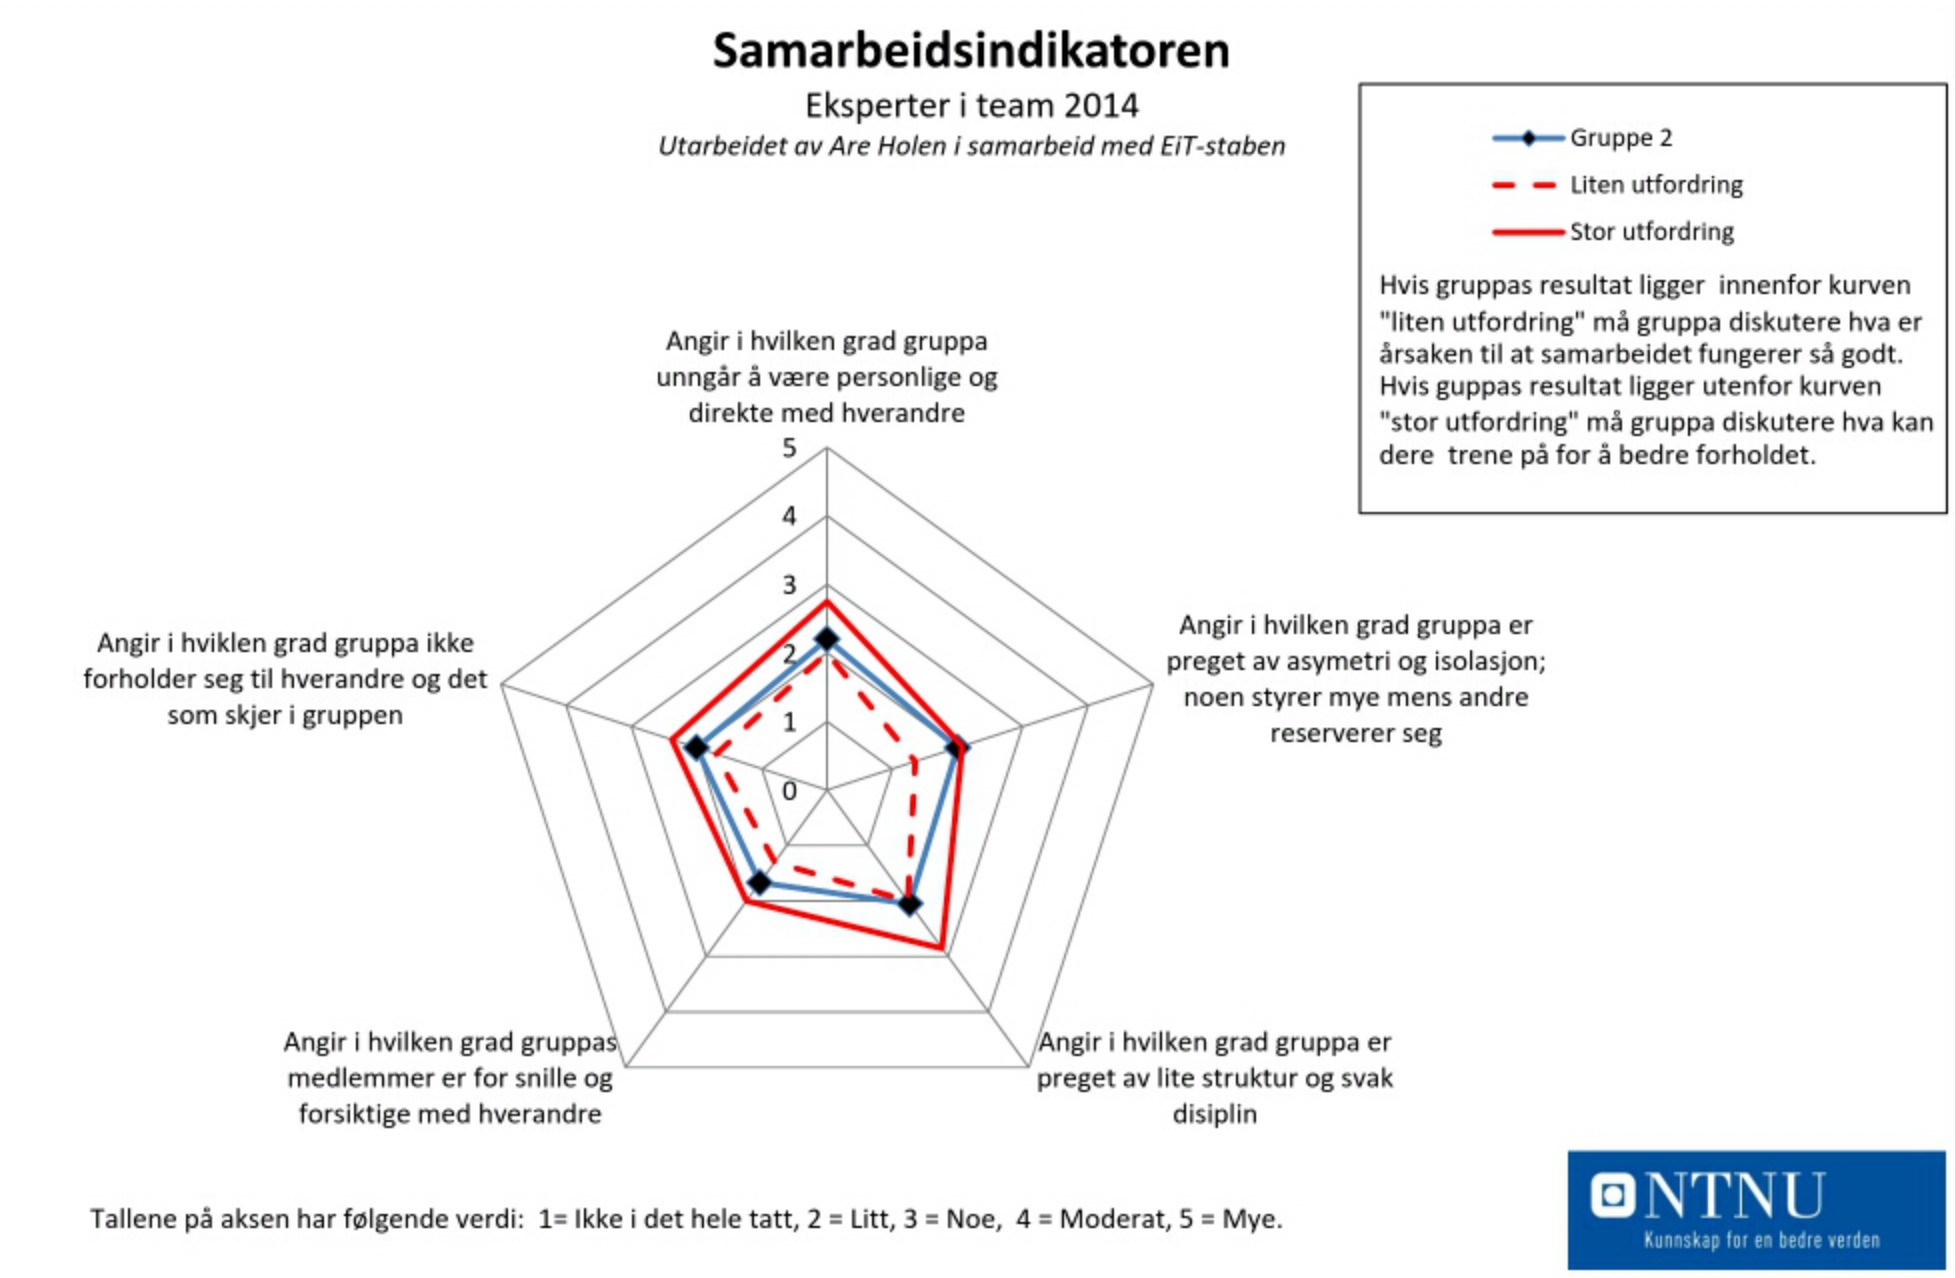
\includegraphics[width=0.7\textwidth]{images/samarbeidsindikator1.jpeg} 
    \caption{Samarbeidsindikatorer 10. landsbydag}
    \label{fig:sam2}
\end{figure}